\documentclass[FM,RP]{tulthesis}
% tento dokument používá balíky specifické pro XeLaTeX a lze jej přeložit
% jen XeLaTeXem, nemáte-li instalována použitá (komerční) písma, změňte
% nebo vymažte příkazy \set...font na následujících řádcích

\newcommand{\verze}{1.7}

\usepackage{polyglossia}
\setdefaultlanguage{czech}
\usepackage{xevlna}

\usepackage{makeidx}
\makeindex

% fonty
\usepackage{fontspec}
\usepackage{xunicode}
\usepackage{xltxtra}
\usepackage{graphicx}
\usepackage{pdfpages} 
\usepackage{wrapfig}

% příkazy specifické pro tento dokument
\newcommand{\argument}[1]{{\ttfamily\color{\tulcolor}#1}}
\newcommand{\argumentindex}[1]{\argument{#1}\index{#1}}
\newcommand{\prostredi}[1]{\argumentindex{#1}}
\newcommand{\prikazneindex}[1]{\argument{\textbackslash #1}}
\newcommand{\prikaz}[1]{\prikazneindex{#1}\index{#1@\textbackslash #1}}
\newenvironment{myquote}{\begin{list}{}{\setlength\leftmargin\parindent}\item[]}{\end{list}}
\newenvironment{listing}{\begin{myquote}\color{\tulcolor}}{\end{myquote}}
\sloppy

% deklarace pro titulní stránku

\TULtitle{Vytvoření výukové aplikace řešící blokové diagramy bezporuchovosti (RBD)}{}
\TULprogramme{B2646}{Informační technologie}{}
\TULbranch{1802R007}{Informační technologie}{}
\TULauthor{Jan Špecián}
\TULsupervisor{Ing. Josef Chudoba, Ph.D.}
\TULyear{2019}

\begin{document}
%\ThesisStart{pic/zadaniBPScan.pdf}
\ThesisStart{male}
%\includepdf[scale=1,angle=0,pages=-]{pic/prohlaseni.pdf} 

\begin{abstractCZ}
    Práce je zaměřena na tvorbu desktopové aplikace v .NET Frameworku pro tvorbu RBD diagramů a s tím spojených výpočtů a vizualizací.
    Výsledná aplikace by měla být schopna dle uživatelem zadaného schématu funkčních bloků s definovanými parametry 
    spočítat pravděpodobnost bezporuchového provozu, že výrobek se do času t nedostane do poruchového stavu.
\end{abstractCZ}

\begin{keywordsCZ}
    Blokový diagram spolehlivosti, Pravděpodobnost poruchy, Intenzita poruch
\end{keywordsCZ}

\begin{abstractEN}
    The work is focused on creating a desktop application in .NET Framework for creating RBD diagrams and related calculations and visualizations.
    Software application as result of the work should be able to follow a user-defined function block diagram with predefined parameters and should be able
    to calculate the probability of non-failure operation ability of the product or system.
\end{abstractEN}

\begin{keywordsEN}
    Reliability block diagram, Probability of failure, Reliability engineering
\end{keywordsEN}

\vspace{2cm}



\clearpage

\begin{acknowledgement}
    Tímto bych rád poděkoval Ing. Josef Chudobovi, Ph.D. za věnovaný čas v konzultacích a odborné vedení plné trpělivosti a s tím spojené nabyté zkušenosti.
\end{acknowledgement}

\tableofcontents
\listoffigures

\clearpage

\begin{abbrList}
    \textbf{RBD} & Reliability Block Diagram \\
    \textbf{WPF} & Windows Presentation Foundation \\
    \textbf{GUI} & Graphical User Interface \\
    \textbf{CLI} & Command Line Interface \\
   
\end{abbrList}

\chapter*{Úvod}
    U každého systému je velmi důležitá jeho funkční spolehlivost během doby jeho životnosti. 
    Každý systém, pokud má existovat a fungovat co nejdéle a přitom bez poruch,
    nebo alespoň s jejich co nejmenším počtem, musí splňovat jednu zásadní vlastnost, a tou je spolehlivost. 
    Požadavek na dostatečně velkou a často až maximální spolehlivost námi užívaných systémů má tudíž zcela zásadní význam z hlediska bezpečnostního, ekonomického i
    ekologického. 

    Cílem ročníkového projektu je navrhnout a implementovat desktopovou aplikaci pro tvorbu a jednoduchou vizualizaci RBD diagramů a výpočet parametrů spolehlivosti.
    Aplikace by měla být schopna spočítat dobu do poruchy, či pravděpodobnost bezporuchového provozu za zadané období pro každou komponentu zvlášť a i pro celkový, uživatelem
    nadefinovaný systém. Dále navrhnout další možnosti rozvoje aplikace.

\chapter{Teoretický úvod}
        
    \section*{Distribuční funkce spojité náhodné veličiny}
        Jedním z prostředků pro popis náhodné veličiny je distribuční funkce, která každému
        reálnému číslu přiřazuje pravděpodobnost, že náhodná veličina nabude hodnoty menší nebo
        rovné než toto číslo.\cite{6}
        U spojité náhodné veličiny se užívá k jejímu popisu distribuční funkce F(t) definované vztahem: 
        $$ F(t_{i}) = P(T<t_{i}) $$
            \begin{figure}[h]
                \centering
                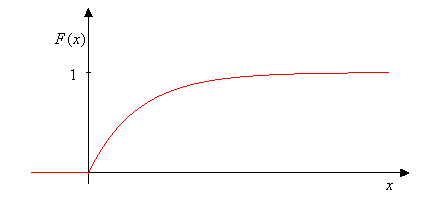
\includegraphics[scale=0.75]{pic/distrib.png}
                \caption{Příklad průběhu distribuční funkce exponenciálního rozdělení} 
            \end{figure}
        \subsubsection*{Vlastnosti distribuční funkce}
            \begin{itemize} 
                \item
                Hodnoty distribuční funkce leží v intervalu od nuly do jedné.
                $$ 0 \leq F(x) \leq 1 $$
                \item
                Distribuční funkce je neklesající.
                $$  P(x_{1} \leq X < x_{2}) = F(x_{2}) - F(x_{1}) \mbox{ pro }x_{1} < x_{2} $$
                \item
                V záporném nekonečnu se blíží k nule, v kladném nekonečnu se blíží k jedné.
                $$ F(- ∞) = 0, F(∞) = 1 $$ 
            \end{itemize}

    \section*{Spolehlivost a střední doba mezi poruchami}
        \subsubsection*{Střední doba mezi poruchami}
            Základní veličinou pro měření spolehlivosti systému je střední doba mezi poruchami (MTBF, Mean Time
            Between Failure). Obvykle je udávána v hodinách. Čím vyšší je hodnota MTBF, tím vyšší je spolehlivost
            produktu.\cite{3}
            Je statistická veličina používaná ke kvantifikaci spolehlivosti součásti, či celého výrobku.
            Určuje se pro výrobek nebo zařízení, které se opravuje. \cite{3}
        \subsubsection*{Spolehlivost}
            Spolehlivost je schopnost systému nebo součásti vykonávat požadované funkce za daných
            podmínek po určené časové období \cite{1} 

            %$$ Spolehlivost = e^{-(\frac{Doba}{MTBF})}$$

        \subsubsection*{Pravděpodobnost bezporuchovosti}
            Značíme $ R(t) $. Udává pravděpodobnost, že výrobek do zadaného času $ t $ nebude mít poruchu. Jedná se o doplněk k hodnotě distribuční funkce $ F(t) $,
            což udává pravděpodobnost, že výrobek bude mít do času $ t $ poruchu.\cite{5}

            Pravděpodobnost bezporuchového provozu R(t) je dána vztahem:
            $$ R(t)=1-F(t) $$

            Pro výpočet pravděpodobnosti bezporuchového provozu se nejčastěji používá exponenciální rozdělení.

    \section*{Exponenciální rozdělění}
        Toto rozdělení má spojitá náhodná veličina X, která představuje dobu čekání do nastoupení (poissonovského) náhodného jevu, 
        nebo délku intervalu (časového nebo délkového) mezi takovými dvěma jevy (např. doba čekání na obsluhu, vzdálenost mezi dvěma poškozenými místy na silnici, doba do poruchy).
        Závisí na parametru $ \lambda $, což je převrácená hodnota střední hodnoty doby čekání do nastoupení sledovaného jevu. \cite{6}

        Náhodná veličina X má exponenciální rozdělení Exp($ \lambda $) právě tehdy, když platí:
        \subsubsection*{Hustota pravděpodobnosti}
        $  f(t) = \left\{ \begin{array}{ll}
            0 & \mbox{pro }t<0 \\
            \lambda.e^{\lambda.t} & \mbox{pro }t\geq 1
            \end{array} \right. $
            \begin{figure}[h]
                \centering
                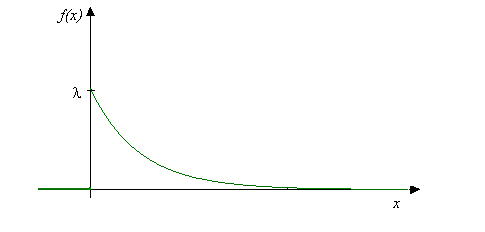
\includegraphics[scale=0.75]{pic/hustota.png}
                \caption{Příklad grafu hustoty pravděpodobnosti exponenciálního rozdělení} 
            \end{figure}
        \subsubsection*{Distribuční funkce}
            $  F(t) = \left\{ \begin{array}{ll}
                0 & \mbox{pro }t<0 \\
                1-e^{-\lambda.t} & \mbox{pro }t\geq 1
                \end{array} \right. $
            \begin{figure}[h]
                \centering
                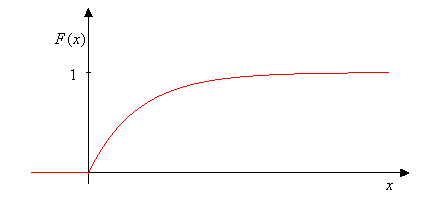
\includegraphics[scale=0.75]{pic/distrib.png}
                \caption{Příklad průběhu distribuční funkce exponenciálního rozdělení} 
            \end{figure}
        \subsubsection*{Střední hodnota}
            $$ E(t) = \frac{1}{\lambda}  $$
        

    
   
    \section*{Analýza blokového diagramu bezporuchovosti (RBD)}

        Analýza blokového diagramu bezporuchovosti (RBD - Reliability Block Diagram) je metoda analýzy systému. 
        Diagram RBD je grafická reprezentace logické struktury systému v podobě podsystémů, nebo jednotlivých součástí. 
        To umožňuje, aby byly cesty úspěchu (funkceschopného stavu) reprezentovány tak, jak jsou bloky (podsystémy/součásti) logicky propojeny.\cite{1}

        Blokové diagramy jsou mezi prvními úkoly dokončenými během etapy vymezení produktu. 
        Mají být vypracovány jako součást vývoje počáteční koncepce. 
        Práce na nich mají být zahájeny, jakmile existuje vymezení programu, a mají být dokončeny jako součást analýzy požadavků a 
        mají se neustále rozšiřovat do větších úrovní podrobnosti, 
        jakmile budou k dispozici data, aby bylo možné činit rozhodnutí a provádět optimalizace nákladů a přínosů.\cite{2}

    \section*{Základní zapojení bloků}
        \subsubsection*{Sériové zapojení}
            Při poruše jedné komponenty dojde k poruše celého systému. 
            Systém je v bezporuchovém stavu, pokud všechny jeho komponenty nemají poruchu.\cite{5}
            Pravděpodobnost bezporuchového provozu (n) zařízení v sériovém systému je dána vztahem:
            $$ R = R_{1}R_{2}...R_{n} = e^{-\lambda_{1}t}e^{-\lambda_{2}t}...e^{-\lambda_{n}t} = e^{-(\lambda_{1} + \lambda_{2} + ... +\lambda_{n})t} $$
            \begin{figure}[h]
                \centering
                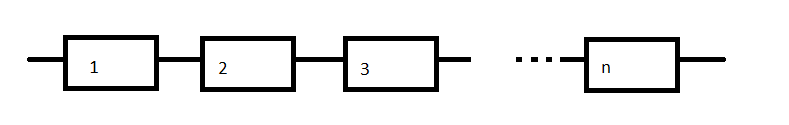
\includegraphics[scale=0.75]{pic/seriove.png}
                \caption{Příklad sériového zapojení komponent} 
            \end{figure}
            \begin{wrapfigure}{r}{265pt}
                \begin{center}
                    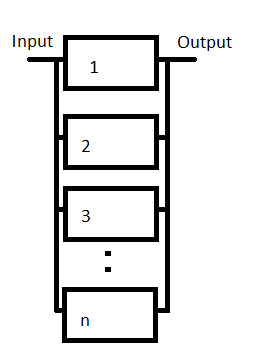
\includegraphics[scale=0.75]{pic/paralelni.png}
                    \caption{Příklad paralelního zapojení kopmonent} 
                \end{center}
            \end{wrapfigure}
        \subsubsection*{Paralelní zapojení}
            K poruše celého systemu dochází pokud jsou v poruše všechny jeho komponenty. Bezporuchový stav trvá, dokud je alespoň jedna komponenta v bezporuchovém stavu.
            
            Z hlediska odhadu pravděpodobnosti představuje paralelní systém nejlepší variantu pro odhad pravděpodobnosti bezporuchového stavu. \cite{5}
            Pravděpodobnost, že všechny komponenty (n) v paralelním systému budou mít poruchu je dána vztahem:
            $$ F = F_{1}F_{2}...F_{n} = (1-e^{-\lambda_{1}t})(1-e^{-\lambda_{2}t})...(1-e^{-\lambda_{n}t}) $$



\chapter{Přehled existujících softwarových nástrojů}
    Zde uvedu seznam existujících softwarových řešení pro výpočty v oblasti pravděpodobnosti a teorie spolehlivosti, jejichž prospekty a ukázky jsem prošel.
    \begin{itemize} 
        \item ReliaSoft - analýza spolehlivosti, www.reliasoft.com. \cite{8}
        \item Weibull.com - Reliability Analysis Software, www.weibull.com. \cite{9}
        \item ItemSoft - Reliability Engineering Software, www.itemsoft.com. \cite{10}
        \item AldService - Reliability Engineering, www.aldservice.com. \cite{11}
        \item Bqr - Leader in Reliability \& Maintenance Engineering and EDA, www.bqr.com. \cite{12}
        \item Goldsim - Reliability Engineering and Risk Analysis for Complex Engineered Systems,www.goldsim.com. \cite{13}
        \item R Project - free software environment for statistical computing and graphics, www.r-project.org. \cite{14}
    \end{itemize}

\chapter{Návrh desktopové aplikce .NET}
    \section*{Objektová struktura}
        \begin{figure}[h]
        \centering
        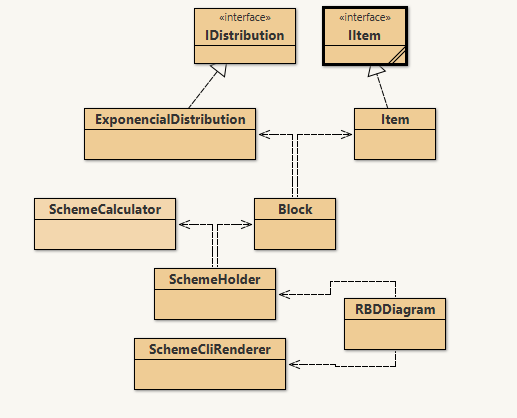
\includegraphics[scale=0.85]{pic/class.png}
        \caption{Zjednodušený class diagram nejčastěji používaných objektů} 
    \end{figure}
        \subsubsection*{IDistribution a ExponencialDistribution}
            Rozhraní pro rozdělení pravděpodobnosti, které je jedním z atributů objektů typu Item.
            Objekty imlementující toto rozhraní musí umět poskytnout střední hodnotu, hodnotu distribuční funkce v daném bodě, hodnotu pravděpodobnostní funkce v daném bodě.
            Jedním z implementujících tříd rozhraní IDistribution je ExponencialDistribution. Instance této třídy reprezentuje konkrétní exponenciální 
            rozdělení pravděpodobnosti se zadaným parametrem $ \lambda $.
        \subsubsection*{Item}
            Pro reprezentaci jednoho bloku diagramu byla navržena třída Item. Její instance jsou objekty reprezentující jeden prvek diagramu, například na obrázku č. 1.4 block číslo 1. 
            Obsahuje dva hlavní atributy a tím je objekt exponenciálního rozdělelní pravděpodobnosti, jméno a další atributy.
            Na základě předaného rozdělení se každého objektu dotázat na hodnoty jeho distribuční funkce. Tyto hodnoty jsou použity pro výpočet pravděpodobnosti bezporuchovosti.
        \subsubsection*{Block}
            Jedná se o hlavní stvební stavební prvek v sériově-paralelním RBD diagramu.
            Může reprezentovat pouze jednu komponentu, či kolekci paralelních komponent typu Item. 
            Tyto bloky jsou spojovány do série za sebe.
            Instance třídy Block reprezentuje například bloky č. 4 a 6 na obrázku č. 4.1.
        %\begin{wrapfigure}{l}{265pt}
        %    \begin{center}
        %        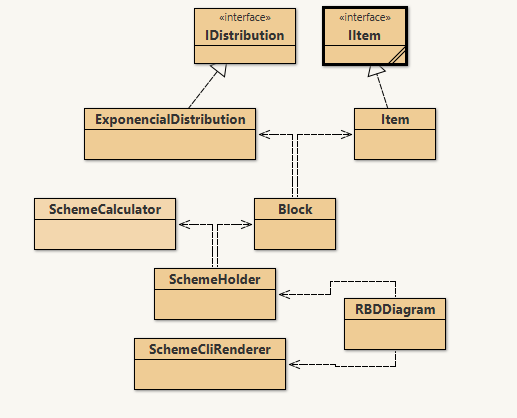
\includegraphics[width=250pt]{pic/class.png}
        %        \caption{Zjednodušený class diagram nejčastěji používaných objektů}
        %    \end{center}
        %\end{wrapfigure}
    
    \section*{Pomocné třídy}
        SchemeHolder je objekt držící jednotlivé bloky v seznamu, tak jak byly vloženy. Přidávané bloky řadí za sebe do spojového seznamu.
        SchemeCalculator je servisní třída, která má za úkol na základě předaných parametrů na uloženém schématu spočítat dílčí pravděpodobnosti bezporuchovosti jednotlivých komponent,
        tak i celkového diagramu. Této třídy se uživatelské rozhraní dotazuje na hodnoty pravděpodobnosti. 

\chapter{Průběh vývoje}
    Pro vývoj jsem se rozhodl použít WinForms z .NET Frameworku, jelikož umožňuje jednoduchou tvorbu formulářových aplikací pomocí grafického designeru.
    Objektová struktura pro uložení diagramu je složena ze seznamu objeků typu Block. Tyto objekty lze řadit za sebe do série.

    \section*{Zjednodušení diagramu}
        Pro zjednodušení tvorby diagramu bylo zavedeno pravidlo, že se systém skládá pouze ze série bloků, z nichž některé mohou reprezentovat paralelní zapojení.
        V aplikaci nelze vytvořit diagram obsahující vazby mezi bloky, které spolu bezprostředně nesousedí. Na obrázku č. 4.1 vidíme typ diagramu, jaký lze vytvořit.
        \begin{figure}[h]
          \centering
           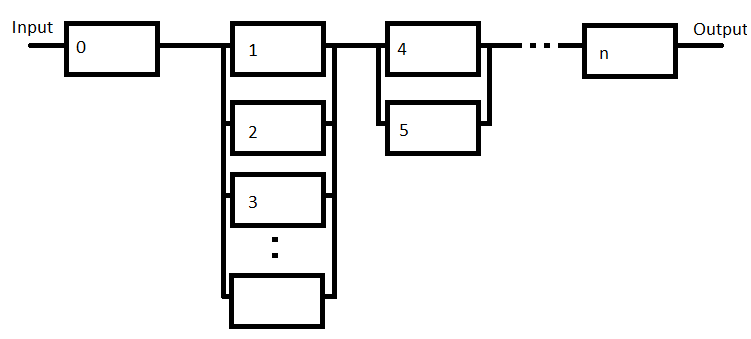
\includegraphics[scale=0.55]{pic/moznosti.png}
           \caption{Možnosti tvorby diagramu} 
        \end{figure}

    \section*{Rozdělení projektu na subprojekty}
        Celkové řešení je rozděleno na několik podprojektů, tak aby každý odpovídal svému účelu použití.
        \begin{itemize} 
        \item SpecianPRJ - projekt obsahující veškeré objektové struktury.
        \item SpecianPRJ.Cli - projekt zaměřený na manuální testování navržených struktur.
        \item SpecianPRJ.Gui - grafické uživatelské rozhraní pro výslednou aplikaci.
        \item SpecianPRJ.Tests - unit testy pro výpočty pravděpodobnosti na exponenciálním rozdělení.
        \end{itemize}

    \section*{Testování}
        Pro testování funkčních bloků byla použita výchozí knihovna pro Unit testování v prostředí .NET pro desktopové aplikace MSTest.
        %Za pomoci testování jsem došel ke správným výsledkům za pomoci připravené konfigurace a tím jsem ušetřil práci manuálním testováním.
                \begin{wrapfigure}{l}{265pt}
            \begin{center}
                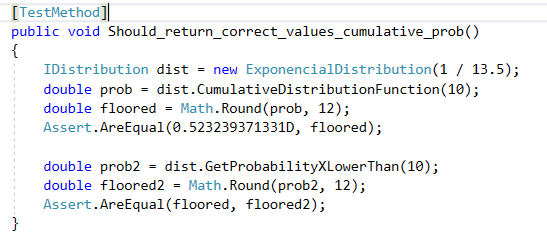
\includegraphics[width=250pt]{pic/testMethod.png}
                \caption{Ukázka kódu unit testu}
            \end{center}
        \end{wrapfigure}
        Nespornou výhodou testování je odhalení chyb při změně tím, že testovací metody odhalí neočekávané výledky.
        Pomocí unit testů bylo vyzkoušeno, zda třída ExponencialDistribution vrací správné hodnoty při zadaném parametru $ \lambda $, 
        kterými jsou například střední hodnota, či hodnota distribuční funkce $ F(t) $. Porovnání výstupních hodnot probíhá po zaokrouhlení na 12 desetinných míst.

        \subsection*{Příklad testu}
            Mějme veličinu s exponenciálním rozdělením a s střední hodnotou 13,5. Pak $\lambda = 1 / 13.5 \approx 0,074074 $.
        %\begin{figure}[h]
         % \centering
          % 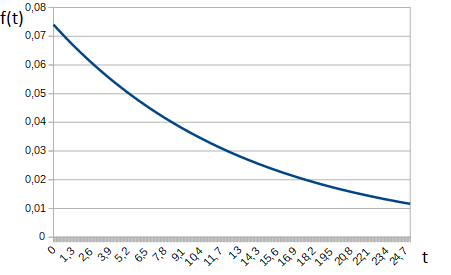
\includegraphics[scale=0.75]{pic/testHustota.png}
           %\caption{Hustota pravděpodobnosti exponenciálního rozdělení se střední hodnotou 1/13.5} 
        %\end{figure}

        \begin{wrapfigure}{l}{265pt}
            \begin{center}
                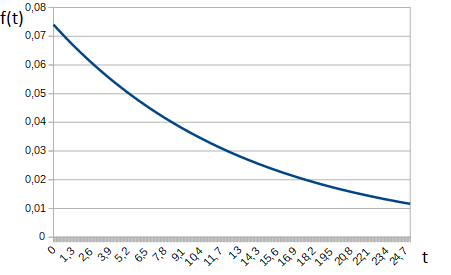
\includegraphics[width=250pt]{pic/testHustota.png}
                \caption{Hustota pravděpodobnosti exponenciálního rozdělení se střední hodnotou 13.5}
            \end{center}
        \end{wrapfigure}

            Na obrázku č. 4.2 vidíme test, zda-li třída vrátí správnou hodnotu, pokud chceme vědět, jaká je pravděpodobnost, že $ t < 10 $.

        %\begin{figure}[h]
        %  \centering
        %   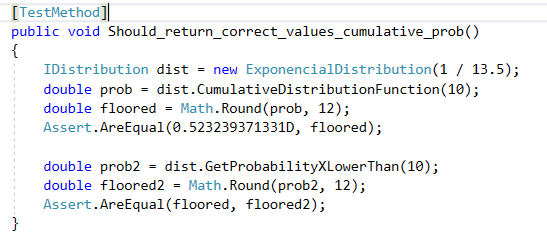
\includegraphics[scale=0.75]{pic/testMethod.png}
        %   \caption{Ukázka kódu unit testu} 
        %\end{figure}

\chapter{Návod k použití}

    Pro spuštění aplikace pro vývoj je potřeba mít nainstalované Visual Studio 2017 a novější. 
    V přiloženém CD ve složce SpecianPRJ spusťte soubor SpecianPRJ.sln. 

    Pro standartní spuštění aplikace stačí otevřít soubor SpecianPRJ.Gui.exe ve složce \path{SpecianPRJ\SpecianPRJ.Gui\bin\Debug}

    Pro obě varianty spuštní je nutným předpokladem nainstalovaný plný .NET Framework 4.6.1 a novější. 
    \begin{figure}[h]
        \centering
        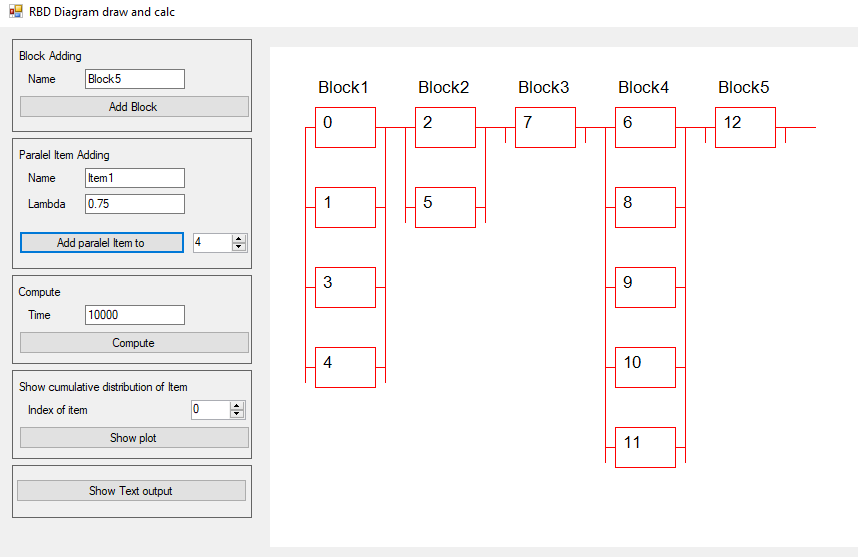
\includegraphics[scale=0.70]{pic/gui.png}
        \caption{Ovládací panel grafického uživatelského rozhraní se zadaným diagramem} 
    \end{figure}
    \subsection*{Založení nového diagramu}
        V současné podobě aplikace je nový diagram založen při každém spuštění aplikace. Jedná se o prázný seznam bloků v instanci SchemeHolder.
    %\section*{Uložení a otevření nového diagramu}
    \subsection*{Přidání prvku}
        Pomocí ovládacích prvků lze přidat bloky a do nich jednotlivé paralelní komponenty. 
        Blok může reprezentovat jedna, či více komponent typu Item.
    \subsection*{Výpočty}
        Uživatel po nadefinování schématu se může dotázat na pravděpodobnost bezporuchovosti v zadaném čase pro zadané schéma.
        Dále lze zobrazit průběh distribuční funkce pro libovonlý blok v separátním okně, za pomoci knihovny OxyPlot \cite{15}
    \subsection*{Ukázka použití}
        Na obrázku č. 5.1 vidíme hlavní okno aplikace. Po pravé straně je ovládací panel pro přidvání položek do diagramu.
        Na obrázku č. 5.2 vidíme vedlejší okno s průběhem distribuční funkce vybrané komponenty.
    \begin{figure}[h]
        \centering
        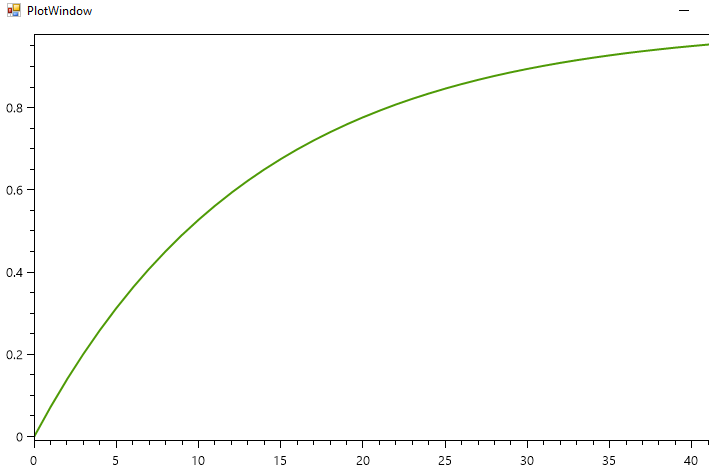
\includegraphics[scale=0.50]{pic/oxy.png}
        \caption{Distribuční funkce exponenciálního rozdělení pro položku s indexem 1} 
    \end{figure}
    \begin{figure}[h]
        \centering
        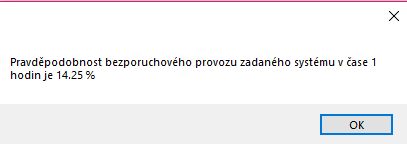
\includegraphics[scale=0.8]{pic/hlaska.png}
        \caption{Pravděpodobnost bezporuchovosti zařízení znázorněné diagramem na obrázku č. 5.1 V tomto příkladu mají všechny komponenty: $ \lambda = 0.75 $} 
    \end{figure}


\chapter{Závěr}

    Byla navrhnuta jednoduchá objektová struktura, na níž lze spočítat pravděpodobnost bezporuchovosti, 
    distribuční funkci pro exponenciální rozdělení a další potřebné charakteristiky.
    Ve vývojovém studiu Microsoft Visual Studio byl vytvořen projekt s rozdělenou strukturou podprojektů pro grafické rozhraní, objektovou stukturu a testování.

    Na základě této objektové struktury jsem navrhl grafické rozhraní za pomoci knihoven WinForms, 
    ve kterém uživatel aplikace snadno nadefinuje strukturu komponent v sérii a může se na definovanou strukturu dotázat
    na pravděpodobnost bezporuchovosti v zadaném čase. 
    Správnost výpočtů pravděpodobností a hodnot distribuční funkce byla otestována za pomoci unit testů.

    Tvorba a zapojení komponent v RBD diagramu bylo zjednodušeno na sériově-paralelní systém, kde jednotlivé bloky jsou v sérii 
    a každý jednotlivý blok může obsahovat několik paralelních komponent.

    Při vývoji aplikace jsem používal verzovací nástroj git, který mi umožnil si v různých větvích držet různé funkční a nefunkční cesty vývoje a spojovat do sebe různé
    věvte pro dosažení funkčního celku. \cite{7}

    Vykreslení schématu do plochy ovládacího okna probíhá za pomoci geometrických primitiv a jejich skládání. 
    Konkrétně se jedná o úsečky a textová pole s indexem komponenty.
    ro zobrazení distribučních funkcí jednotlivých komponent diagramu byla použita knihovna OxyPlot. 
    Pro určení maxima na vodorovné ose byl použit 95 procentní kvantil.
    Veškeré výstupy jsou dostupné i v textové podobě.

    Pro možnost složitějších diagramů by bylo nutné předělat objektový model včetně výpočetního postupu tak, aby paralelní bloky mohly být opět jiné objekty typu Block.
    Dále by bylo vhodné k aplikaci přidat možnost uložení a znovuotevírání uložených diagramů,
    nyní je aplikace pouze demonstrační a diagram je nutné manuálně vytvořit po spuštění.

    Pro grafické uživatelské rozhraní by bylo vhodné přejít na knihovny WPF, které jsou nástupcem zastaralých Windows Forms.

\begin{thebibliography}{Mm99}
    \bibitem{1}
        Analýza stromu událostí (ETA). Www.qmprofi.cz [online]. 2007 [cit. 2019-05-01]. Dostupné z: https://www.qmprofi.cz/33/analyza-stromu-udalosti-eta-uniqueidmRRWSbk196FNf8-jVUh4EuiqB7MU5EZkI4KJhlhjbS2LV4wcZRqCHQ/
    \bibitem{2}
        NOVÁK, Bc. Rudolf. Analýza spolehlivosti v oblasti IT. 2009. Diplomová práce. JIHOČESKÁ UNIVERZITA V ČESKÝCH BUDĚJOVICÍCH. Vedoucí práce Ing. Ludvík Friebel, Ph.D.
    \bibitem{3}
        TORELL, Wendy. Střední doba mezi poruchami: vysvětlení a standardy. Http://gabben.wbs.cz [online]. [cit. 2019-05-01]. Dostupné z: http://gabben.wbs.cz/mtbf1.pdf
    \bibitem{5}
        PAVEL, Fuchs, CSc. a Vališ, Ph.D. DAVID. Bezporuchovost a životnost: Techniky analýzy bezporuchovosti.
    \bibitem{6}
        OTIPKA, Petr a Vladislav ŠMAJSTRLA. PRAVDĚPODOBNOST A STATISTIKA [online]. VYSOKÁ ŠKOLA BÁŇSKÁ - TECHNICKÁ UNIVERZITA OSTRAVA [cit. 2019-05-01]. Dostupné z: https://homen.vsb.cz/~oti73/cdpast1/
    \bibitem{7}
        We bring the awesome Git SCM to Windows. Git for windows [online]. [cit.2019-04-24]. Dostupné z: https://gitforwindows.org/
    \bibitem{8}
        ReliaSoft. ReliaSoft [online]. [cit. 2019-05-07]. Dostupné z: https://www.reliasoft.com/
    \bibitem{9}
        Reliability Engineering Resource Website. Weibull.com [online]. [cit. 2019-05-07]. Dostupné z: https://weibull.com/
    \bibitem{10}
        Item software. Item software [online]. [cit. 2019-05-07]. Dostupné z: http://www.itemsoft.com/
    \bibitem{11}
        RAMS (Reliability, Availability, Maintainability and Safety) Software. Reliability Software, Safety and Quality Solutions - ALD Service [online]. [cit. 2019-05-07]. Dostupné z: https://aldservice.com/reliability-products/rams-software.html
    \bibitem{12}
        BQR Reliability Engineering. BQR - Leader in Reliability \& Maintenance Engineering and EDA [online]. [cit. 2019-05-07]. Dostupné z: https://www.bqr.com/
    \bibitem{13}
        GoldSim: Monte Carlo Simulation Software. GoldSim Technology Group [online]. [cit. 2019-05-07]. Dostupné z: https://www.goldsim.com/Web/Products/GoldSim/Overview/
    \bibitem{14}
        The R Project for Statistical Computing. The R Project [online]. [cit. 2019-05-07]. Dostupné z: https://www.r-project.org/
    \bibitem{15}
        OxyPlot’s documentation. OxyPlot [online]. [cit. 2019-05-07]. Dostupné z: https://www.oxyplot.org/
\end{thebibliography}

\end{document}
